%!TEX root = TIHSC_Project_main.tex
\chapter{SystemC TLM}
The transaction level model (TLM) for a systemC model is good for validating and verifying the model. 

Throughout this project an application in C/C++ is available. The challenge is then to allocate and bind the different parts to either software or hardware. 
With a TLM it is possible to investigate different mappings before implementation. 
%Because of the known application some kind of execution time is also known. This makes it possible to prioritise the modelling of the components. 

In the TLM a CPU and the k-means is made as a systemC module. Inside the CPU module three threads are deployed. One for reading in the image, one for writing out the image and one for doing the texton filtering. 
The k-means module has one thread for doing the classification on the filtered image, see figure \ref{fig:TLM}.

\begin{figure}[H]
\centering
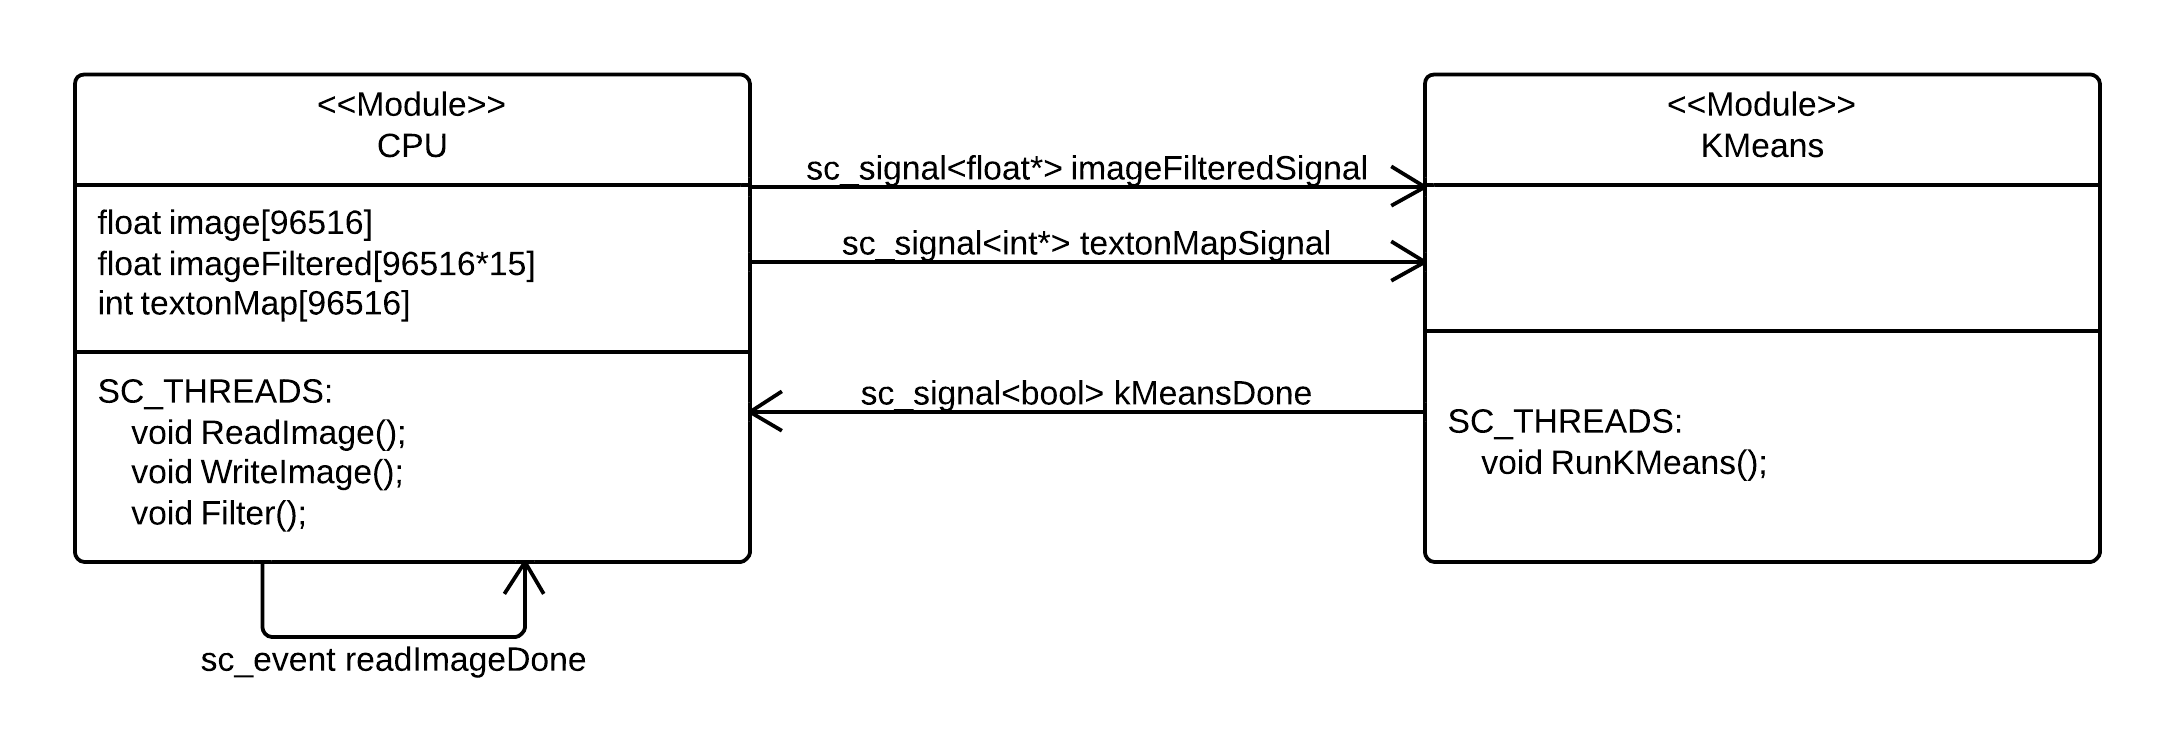
\includegraphics[width = \linewidth]{SystemCModuleDiagram}
\caption{SystemC module diagram}
\label{fig:TLM}
\end{figure}

Memory is not considered in the TLM. Between the two modules a lot of data is transferred. 
As seen in figure \ref{fig:TLM} signals between the modules represents pointers to the arrays created in the CPU module. 

